\documentclass[sans]{beamer}

\mode<presentation>
{
	% \usetheme{CambridgeUS}
	% \usetheme{Hannover}
	\usetheme{Singapore}
	\usecolortheme{default}
}

\usepackage{cmap}
\usepackage{listings}
\usepackage{lmodern}
\usepackage{color}
\usepackage{minted}
\usepackage{graphicx}
\usepackage{tikz}
\usepackage{wrapfig}

\usepackage[labelformat=empty]{caption}
\usepackage{fontspec}
\usepackage{polyglossia}
\setdefaultlanguage{russian}

\setmainfont[Ligatures=TeX]{DejaVu Serif}
\setsansfont[Ligatures=TeX]{DejaVu Sans}
\setmonofont{DejaVu Sans Mono}

\definecolor{myGray}{RGB}{50,50,50}

\begin{document}
\title
[Форматирование программ]
{Форматирование программ

\small
Принтер-комбинаторы и сопоставление с образцом}
\author
[Подкопаев Антон]{Подкопаев Антон, \texttt podkoav239@gmail.com}
\institute{Лаборатория JetBrains}
\date [27-03-14]{27 марта 2014}

\begin{frame}[plain]
	\titlepage
\end{frame}

\begin{frame}{Контекст задачи}
  Языковые процессоры

  \begin{itemize}
		\item Синтаксический анализ
		\item Преобразование
		\item Представление результата
		\begin{itemize}
			\item \textcolor{red}{Код программы}
			\item ...
		\end{itemize}
	\end{itemize}

  \pause
  \textcolor{red}{Форматирование кода в IDE}
\end{frame}

\section{Принтер-комбинаторы}

\begin{frame}{Критерии красоты кода}
  % TODO
  TODO
\end{frame}

\begin{frame}{Комбинаторы}
  — это функции высшего порядка, которые из одних функций строят другие
 
	%\vspace{1cm}

  \begin{center}
  \begin{columns}
		\begin{column}{0.5\linewidth}
      \textcolor{myGray}{
        \scriptsize
        %Возможность принимать функции в качестве аргумента и
        %возвращать их в качестве результата —
        %отличительная черта функциональных языков программирования,
        %в которых комбинаторы являются обычными функциями.
        \begin{itemize}
          \item Элементарные функции
          \item Переход от простого к сложному
          \item Пример: парсер-комбинаторы
          \begin{itemize}
            \scriptsize
            \item symbol
            \item >>=
            \item many
            \item option
          \end{itemize}
          \item \textcolor{gray}{Характерны для функционального программирования}
          \item \textcolor{gray}{См. паттерн "Компоновщик" и GUI-frameworks}
        \end{itemize}
      }
		\end{column}
		\begin{column}{0.5\linewidth}
	    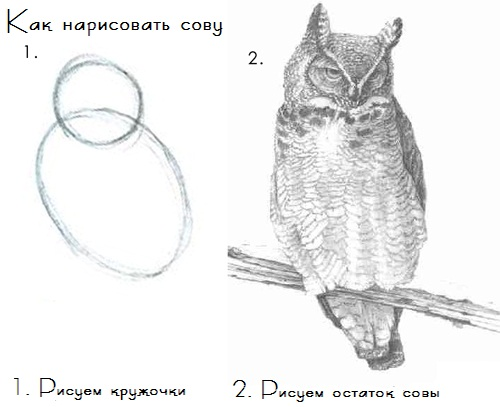
\includegraphics[width = \linewidth]{images/owl.jpg}
		\end{column}
	\end{columns}
  \end{center}
\end{frame}

\begin{frame}{Wadler Doc}
  \inputminted{hs}{codes/wadlerDoc.hs}
\end{frame}

\begin{frame}{Wadler ТТХ}
  \begin{itemize}
    \item Быстро работает \textcolor{gray}{(есть реализации за $O(n)$)}
    \item Не всегда подходит
    \begin{itemize}
      \item Язык Python
        \inputminted{py}{codes/wadlerSeq.py}
    \end{itemize}
  \end{itemize}
\end{frame}

\begin{frame}{Azero, Swierstra Format}
  \inputminted{hs}{codes/swierstraFormat.hs}

  \vspace{0.2cm}

  \begin{columns}
    \begin{column}{0.3\linewidth}
      \centering
      \tikz{
        \draw (0,0) -- (1,0) -- (1,0.2) -- (2,0.2) -- (2,1) -- (0, 1) -- cycle;
      }
    \end{column}
    
    \begin{column}{0.3\linewidth}
      \centering
      \tikz{
        \draw (0,0) -- (1,0) -- (1,0.2) -- (2,0.2) -- (2,1) -- (0, 1) -- cycle;
        \draw (1.1,-0.9) -- (2.1,-0.9) -- (2.1,-0.7) -- (3.1,-0.7) -- (3.1,0.1) -- (1.1,0.1) -- cycle;
      }
    \end{column}

    \begin{column}{0.3\linewidth}
      \centering
      \tikz{
        \draw (0,0) -- (1,0) -- (1,0.2) -- (2,0.2) -- (2,1) -- (0, 1) -- cycle;
        \draw (0,-1.1) -- (1,-1.1) -- (1,-0.9) -- (2,-0.9) -- (2,-0.1) -- (0,-0.1) -- cycle;
      }
    \end{column}
  \end{columns}

  \vspace{0.2cm}

  \begin{columns}
    \begin{column}{0.3\linewidth}
      \centering
      \scriptsize
      Single
    \end{column}
    \begin{column}{0.3\linewidth}
      \centering
      \scriptsize
      Beside
    \end{column}
    \begin{column}{0.3\linewidth}
      \centering
      \scriptsize
      Above
    \end{column}

  \end{columns}
\end{frame}

\begin{frame}{Azero, Swierstra Doc}
  \inputminted{hs}{codes/swierstraDoc.hs}
\end{frame}

\begin{frame}{Azero, Swierstra pretty}
  \inputminted{hs}{codes/swierstraPretty.hs}
\end{frame}

\begin{frame}{Azero, Swierstra ТТХ}
  \begin{itemize}
    \item Работает в худшем случае за $O(e ^ n)$
    \item Выразительная способность достаточная для применения с шаблонами 
    \item Выдает оптимальный результат
    \begin{itemize}
      \item Самый низкий вариант из попадающих в заданную ширину
    \end{itemize}
  \end{itemize}
\end{frame}

\begin{frame}{BURS}
  Bottom-Up Rewrite Systems

  \begin{itemize}
    \item Динамическое программирование на деревьях (дэгах)
    \item Правила
    $$
    \begin{array}{rcll}

      N &:& \alpha& [c]\\
      N &:& \alpha\; (K_1,\dots,K_n)& [c]
    \end{array}
    $$
    \item Нахождение лучшей раскладки за линейное время от размера структуры
  \end{itemize}

\end{frame}

\begin{frame}{Мои комбинаторы}
  \begin{itemize}
    \item Тот же самый интерфейс и результат,
      
      что и у Azero, Swierstra
    \item Факторизация по размерам Format
      \inputminted{hs}{codes/myCombFS.hs}
    \item Ключ Map - нетерминал в BURS
  \end{itemize}
\end{frame}

\begin{frame}{Алгоритмическая сложность}
  $O(w^{p * k} * n)$
  \begin{itemize}
    \item $k$ - максимальная степень дерева (дэга)
    \item $p$ - размерность ключа Map
    \item $w$ - ширина вывода
    \item В случае комбинаторов Beside, Above, Choice
    \begin{itemize}
      \item $k = 2, p = 2$
      \item Сложность: $O(w^4 * n)$ 
    \end{itemize}
    % \item Максимальный размер FormatSet: $m = O(w^2)$
    % \item Сложность операций Beside, Above: $O(m^2)$
  \end{itemize}
\end{frame}

\end{document}
